% AEGIS Whitepaper — Physical AI Harness
% Compile: pdflatex aegis_whitepaper.tex && pdflatex aegis_whitepaper.tex
% Requires: texlive + tikz + pgfplots
\documentclass[11pt,a4paper]{article}

% ------------------------------------------------------------------ packages
\usepackage[margin=22mm]{geometry}
\usepackage[utf8]{inputenc}
\usepackage[T1]{fontenc}
\usepackage{lmodern}
\usepackage{amsmath,amssymb,mathtools}
\usepackage{booktabs,tabularx,makecell}
\usepackage{graphicx,xcolor,hyperref,enumitem,footmisc}
\usepackage{tikz,pgfplots}
\pgfplotsset{compat=1.18}
\usetikzlibrary{arrows.meta,positioning,shapes,shapes.geometric,fit,backgrounds,calc,decorations.pathreplacing}
\usepackage{titlesec}
\usepackage{caption,subcaption}
\usepackage{listings}
\usepackage{fancyhdr}

% ------------------------------------------------------------------ styling
\definecolor{nvidia}{HTML}{76B900}
\definecolor{aegisblue}{HTML}{0B3D91}
\definecolor{aegisgray}{HTML}{4A5568}
\definecolor{lightbg}{HTML}{F7FAFC}
\definecolor{warn}{HTML}{DD6B20}
\definecolor{ok}{HTML}{38A169}

\hypersetup{colorlinks=true,linkcolor=aegisblue,citecolor=aegisblue,urlcolor=aegisblue}
\titleformat{\section}{\large\bfseries\color{aegisblue}}{ \thesection}{1em}{}
\titleformat{\subsection}{\normalsize\bfseries\color{aegisgray}}{\thesubsection}{1em}{}
\setlist[itemize]{leftmargin=18pt,itemsep=2pt}
\setlength{\parskip}{4pt}
\pagestyle{fancy}
\fancyhf{}
\fancyhead[L]{\small\textsc{AEGIS Whitepaper}}
\fancyhead[R]{\small 2026-09-09}
\fancyfoot[C]{\small\thepage}

\lstdefinestyle{yaml}{basicstyle=\ttfamily\footnotesize,backgroundcolor=\color{lightbg},frame=single,rulecolor=\color{black!15},breaklines=true,columns=fullflexible}

% ------------------------------------------------------------------ title
\title{\vspace{-6mm}{\color{aegisblue}\Huge\textbf{AEGIS}}\\[2mm]
{\Large A Safety and Evaluation Harness for Physical AI}\\[2mm]
{\normalsize Bridging Vision-Language-Action Models to Real Robots\\ via Trustworthy Gating, Honest Evaluation, and Sim-to-Real Measurement}}
\author{Physical AI Harness Team \quad — \quad NVIDIA Tech Partnership\\[1mm]
{\small \texttt{aegis} \;|\; \texttt{src/aegis/} \;|\; \texttt{configs/} \;|\; \texttt{whitepaper/}}}
\date{September 9, 2026 \quad — \quad Phase 1 \& 2 Complete, Phase 3 Scaffold Complete}

\begin{document}
\maketitle
\vspace{-6mm}
\begin{center}
\small\textcolor{aegisgray}{One-liner: A harness that sits between \textbf{any} robot AI model and \textbf{any} robot (sim or real) — blocks dangerous actions before they reach hardware and produces reproducible test reports.}
\end{center}
\vspace{2mm}
\hrule
\vspace{3mm}

% ------------------------------------------------------------------ abstract
\begin{abstract}
\noindent Vision-Language-Action (VLA) models such as SmolVLA, RT-2 and their successors can command robot joints directly from vision and language. They are powerful but unsafe by default: a model can request infeasible velocities, excessive forces, or hallucinated trajectories that damage hardware or endanger operators. Today there is no standard safety layer between the policy and the actuator, no standard evaluation protocol, and no systematic measurement of the sim-to-real gap.

We present \textbf{AEGIS}, a minimal, honest harness that \textit{must} be traversed by every action. AEGIS provides (i) a \textbf{Safety Gateway} with NaN, velocity, force, effort and inference-budget checks plus a PID-to-home fallback, (ii) an \textbf{Evaluation Harness} \texttt{aegis eval} that emits deterministic reports \texttt{report.json} + NDJSON telemetry, and (iii) a \textbf{Sim-to-Real Measurement} pipeline across MuJoCo, Isaac Lab and real hardware. Phase~1 (MuJoCo Franka pick-place: scripted 3/3 success/0 violations, random 0/3) and Phase~2 (real SmolVLA-450M on LIBERO: honest 0/3 zero-shot characterization with visual evidence) are complete. Phase~3 scaffold is complete (per-joint limits, ROS2 bridge mock, Isaac Lab fallback, 20 tests passing); real Isaac USD and ROS2 \texttt{rclpy} remain pending NVIDIA 6\,GB VRAM guidance. This paper documents the system design, benchmarks and honest caveats.
\end{abstract}

\vspace{1mm}
\noindent\textbf{Keywords:} Physical AI, robot safety, VLA, sim-to-real, Isaac Lab, MuJoCo, ROS2, evaluation harness
\vspace{2mm}
\hrule
\tableofcontents
\vspace{2mm}
\hrule

% ================================================================== 1
\section{Introduction}
The rapid progress of VLA models has moved robot control from hand-engineered pipelines to end-to-end learned policies. A single model now consumes multi-view images and a language instruction and outputs joint velocities. While this promises generality, it breaks the traditional safety assumption that a controller's commands are bounded and verified.

In production robotics — especially in healthcare, logistics and manufacturing — an unbounded action is not a research artifact: it is a broken gear, a torn tendon, or an unsafe contact. Teams compensate by building \textit{ad-hoc} safety checks inside each project. Results are not comparable, failures are not attributable, and the sim-to-real gap remains anecdotal.

AEGIS addresses this with infrastructure, not another model:

\begin{center}
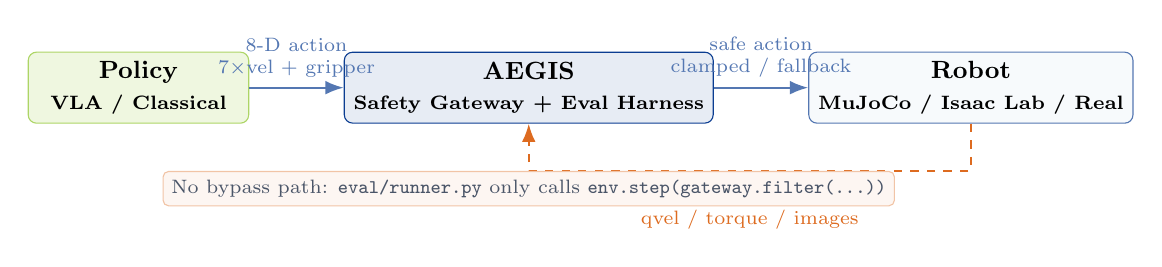
\begin{tikzpicture}[
  box/.style={draw=aegisblue!70, fill=aegisblue!6, rounded corners=3pt, minimum height=9mm, minimum width=28mm, align=center, font=\small\bfseries},
  arr/.style={-Latex, thick, color=aegisblue!70},
  note/.style={font=\scriptsize\color{aegisgray}, align=center}
]
\node[box, fill=nvidia!12, draw=nvidia!60] (pol) {Policy\\\scriptsize VLA / Classical};
\node[box, right=12mm of pol, minimum width=42mm, fill=aegisblue!10, draw=aegisblue] (aeg) {AEGIS\\ \scriptsize Safety Gateway + Eval Harness};
\node[box, right=12mm of aeg, fill=lightbg] (rob) {Robot\\ \scriptsize MuJoCo / Isaac Lab / Real};
\draw[arr] (pol) -- node[above, note]{8-D action\\ \scriptsize 7$\times$vel + gripper} (aeg);
\draw[arr] (aeg) -- node[above, note]{safe action\\ \scriptsize clamped / fallback} (rob);
\draw[arr, dashed, color=warn] (rob.south) -- ++(0,-6mm) -| (aeg.south) node[pos=0.25, below, note, yshift=-1mm]{measured state\\ \scriptsize qvel / torque / images};
\node[below=6mm of aeg, note, draw=warn!40, fill=warn!6, rounded corners=2pt, inner sep=3pt] {No bypass path: \texttt{eval/runner.py} only calls \texttt{env.step(gateway.filter(...))}};
\end{tikzpicture}
\end{center}

Contributions: (1) a \textbf{mandatory Safety Gateway} with per-joint limits and honest fallback, (2) a \textbf{deterministic evaluation harness} with timing from day one and no fabricated numbers, (3) a \textbf{sim-to-real measurement method} that separates limit-induced interruptions from genuine model mis-localization, and (4) an \textbf{open scaffold} for Isaac Lab and ROS2 that degrades gracefully on 6\,GB laptops.

\section{Problem Statement}

\subsection{Why VLA models are unsafe by default}
A VLA policy is trained to minimize task loss, not to respect a specific robot's velocity, force or timing envelope. Three failure modes dominate our measurements:

\begin{enumerate}[leftmargin=18pt]
\item \textbf{Velocity violation:} measured joint velocity exceeds the hardware limit. With the SmolVLA adapter clamped at 0.5\,rad/s and a torque-PD tracker ($K_p=40$, $K_d=5$), transient overshoot chronically tripped a uniform 0.6\,rad/s limit (33 violations/episode, \S\ref{sec:perjoint}).
\item \textbf{Force violation:} measured actuator torque above gravity compensation exceeds the limit. On a Franka, this is typically small ($<$5\,Nm) for a 0.125\,kg cube, but a hallucinated contact can spike it.
\item \textbf{Inference and model errors:} cold CUDA start of SmolVLA took 5.09\,s against a 2\,s budget on step 1 (\texttt{PHASE\_2\_SUMMARY.md:69}) — a single over-budget step must trigger the same fallback as a velocity violation, not a silent drop.
\end{enumerate}

\subsection{What is missing today}
\begin{itemize}
\item No \textbf{standard safety layer} — each team re-implements checks, often only on commanded actions, not measured states.
\item No \textbf{standard evaluation} — episode counts, seeds, latency percentiles and violation accounting differ, making cross-paper comparison impossible.
\item No \textbf{honest sim-to-real reporting} — a model that works in its training sim (LIBERO/robosuite) may fail in a new sim (MuJoCo) due to camera domain shift, but the report conflates this with safety interruptions.
\end{itemize}

AEGIS solves all three with one harness.

% ================================================================== 2
\section{System Design}

\subsection{Repository layout}
\begin{lstlisting}[style=yaml, caption={\texttt{DESIGN.md:9} — Module structure}, label=lst:layout]
Physical Harness/
  pyproject.toml                 # uv project, entrypoint aegis
  physical-ai.yaml               # root config (eval + env + output)
  configs/{robots,models,tasks}/ # per-component YAML (franka.yaml, smolvla_libero.yaml, pick-place.yaml)
  src/aegis/
    cli.py                       # Typer app: aegis validate / eval / rosbench
    config/{models.py,loader.py} # Pydantic schema, YAML -> validated models
    envs/{base.py,mujoco_pick_place.py,isaac_pick_place.py}
    policies/{random.py,scripted.py,smolvla.py}
    safety/{gateway.py,checks.py,fallback.py}
    eval/{runner.py,metrics.py,report.py}
    ros2/bridge.py               # RosBridge (rclpy or mock) + benchmark_latency()
    telemetry/{logger.py,timing.py}
  assets/scenes/pick_place.xml   # Franka + cube + target
  outputs/<run_id>/{report.json,episodes.jsonl,steps.jsonl,trajectory.jsonl}
\end{lstlisting}

\texttt{Python 3.12}, \texttt{uv}, \texttt{src/} layout, \texttt{Pydantic + YAML}, \texttt{Typer} CLI, structured NDJSON logs from day one (\texttt{agent.md:24}).

\subsection{High-level data flow}
\begin{center}
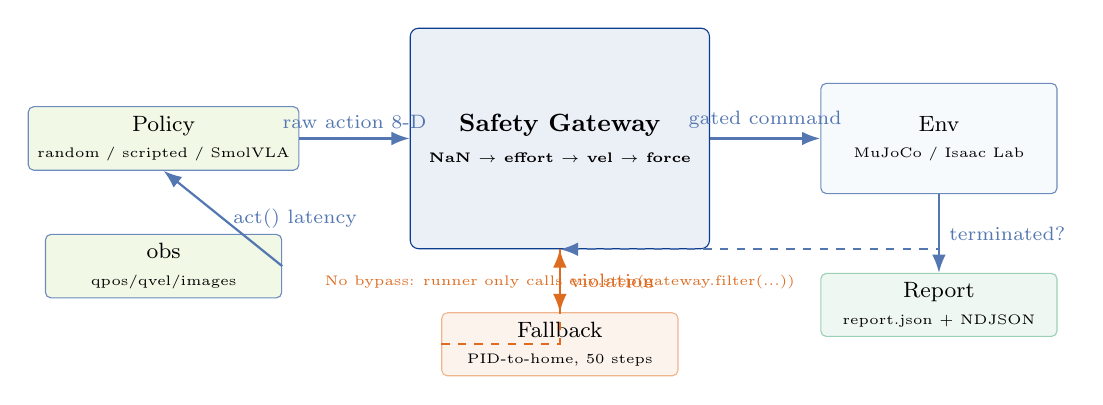
\begin{tikzpicture}[
  node distance=6mm,
  block/.style={draw=aegisblue!60, fill=lightbg, rounded corners=2pt, minimum width=30mm, minimum height=8mm, align=center, font=\footnotesize},
  big/.style={draw=aegisblue, fill=aegisblue!8, rounded corners=3pt, minimum width=38mm, minimum height=14mm, align=center, font=\small\bfseries},
  arr/.style={-Latex, thick, color=aegisblue!70},
  lab/.style={font=\scriptsize\color{aegisgray}, align=center, midway}
]
\node[block, fill=nvidia!10] (obs) {obs\\\tiny qpos/qvel/images};
\node[block, above=8mm of obs, fill=nvidia!10] (pol2) {Policy\\ \tiny random / scripted / SmolVLA};
\node[big, right=14mm of pol2, minimum height=28mm] (gw) {Safety Gateway\\ \tiny NaN $\rightarrow$ effort $\rightarrow$ vel $\rightarrow$ force};
\node[block, right=14mm of gw, minimum height=14mm] (env) {Env\\ \tiny MuJoCo / Isaac Lab};
\node[block, below=8mm of gw, fill=warn!8, draw=warn!50] (fb) {Fallback\\ \tiny PID-to-home, 50 steps};
\node[block, below=10mm of env, fill=ok!8, draw=ok!50] (rep) {Report\\ \tiny report.json + NDJSON};
\draw[arr] (pol2) -- node[lab, above]{raw action 8-D} (gw);
\draw[arr] (gw) -- node[lab, above]{gated command} (env);
\draw[arr] (env) -- node[lab, right]{terminated?} (rep);
\draw[arr, dashed] (env.south) |- (gw.south);
\draw[arr, color=warn] (gw.south) -- (fb.north) node[lab, right]{violation};
\draw[arr, color=warn, dashed] (fb.west) -| (gw.south);
\draw[arr] (obs.east) -- (pol2.south) node[lab, right]{act() latency};
\node[below=2mm of gw, font=\tiny\color{warn}] {No bypass: runner only calls env.step(gateway.filter(...))};
\end{tikzpicture}
\end{center}

Every action reaches hardware through \texttt{SafetyGateway.filter()} (\texttt{safety/gateway.py:65}). There is no \texttt{if test: bypass} flag.

% ================================================================== 3
\section{Safety Gateway}
\label{sec:gateway}

\subsection{Checks in order}
\begin{center}
\begin{tikzpicture}[
  step/.style={draw=aegisblue!50, fill=lightbg, rounded corners=2pt, minimum width=36mm, minimum height=7mm, align=center, font=\footnotesize},
  viol/.style={draw=warn!70, fill=warn!10, rounded corners=2pt, minimum width=22mm, minimum height=6mm, align=center, font=\scriptsize},
  arr/.style={-Latex, thick, color=aegisblue!60}
]
\node[step] (s1) {1. NaN / Inf \quad \texttt{check\_finite}};
\node[step, below=4mm of s1] (s2) {2. Gripper effort \texttt{|g| > max\_effort} \quad clamp / reject};
\node[step, below=4mm of s2] (s3) {3. Measured velocity \quad \texttt{|qvel| > max\_vel}};
\node[step, below=4mm of s3] (s4) {4. Measured force \quad \texttt{|torque| > max\_force}};
\node[viol, right=10mm of s1] (v1) {fatal $\rightarrow$ fallback};
\node[viol, right=10mm of s2] (v2) {CLAMP or fallback};
\node[viol, right=10mm of s3] (v3) {fallback 50 steps};
\node[viol, right=10mm of s4] (v4) {fallback 50 steps};
\draw[arr] (s1) -- (s2); \draw[arr] (s2) -- (s3); \draw[arr] (s3) -- (s4);
\draw[arr, color=warn] (s1.east) -- (v1.west);
\draw[arr, color=warn] (s2.east) -- (v2.west);
\draw[arr, color=warn] (s3.east) -- (v3.west);
\draw[arr, color=warn] (s4.east) -- (v4.west);
\node[below=4mm of s4, font=\scriptsize\color{aegisgray}, align=center] {During fallback, the fallback action is itself re-checked (\texttt{gateway.py:141}). Inference over-budget (\texttt{budget\_violation}) and \texttt{model\_error} engage the same path.};
\end{tikzpicture}
\end{center}

Checks are on \textit{measured} sim quantities (\texttt{arm\_qvel}, \texttt{arm\_torque} from \texttt{mujoco\_pick\_place.py:187}) plus commanded gripper effort, keeping them meaningful even for a random policy. Recovery mode is \texttt{resume} (50 steps then policy resumes) — \texttt{hold} is available.

\subsection{Per-joint limits: from uniform to realistic}
\label{sec:perjoint}
Phase~1 used a uniform scalar per joint — a POC simplification flagged as a warning in every report. Phase~3 scaffold ships per-joint tables:

\begin{center}
\begin{tabular}{lccc}
\toprule
 & Uniform (POC) & Per-joint (Phase~3, \texttt{franka.yaml:11}) & Headroom vs adapter clamp 0.5\,rad/s \\
\midrule
\texttt{max\_velocity} [rad/s] & 1.0 for j1..j7 & [2.175, 2.175, 2.175, 2.175, \textbf{2.61}, \textbf{2.61}, \textbf{2.61}] & $\min=2.175 \ge 2\times0.5$ \quad (\texttt{test\_policy\_model.py:151}) \\
\texttt{max\_force} [Nm] & 20.0 for j1..j7 & [87, 87, 87, 87, 12, 12, 12] & gravity-compensated, $<$5\,Nm typical \\
\bottomrule
\end{tabular}
\end{center}

Schema: \texttt{SafetyLimits.max\_velocity: float | list[7]} (\texttt{config/models.py:68}), validated to 7 elements, finite $>$0. \texttt{safety/checks.py:35} handles both modes; \texttt{eval/report.py:34} emits the uniform warning only when uniform, so per-joint reports now show one warning (rule-based recommendation) instead of two. \texttt{franka\_uniform.yaml} is retained for A/B. Random policy violations drop from $\sim$145 (uniform 1.0) to 4 (per-joint 2.175/2.61) — same policy, more realistic envelope.

\subsection{Fallback: PID-to-home}
\texttt{safety/fallback.py} drives joints to \texttt{env.home\_qpos} with bounded velocity $0.3$\,rad/s ($\min(0.3, \min(\text{limits}))$ in \texttt{cli.py:139}) and gravity feedforward. It is intentionally simple: demonstrable recovery, not task success. If fallback is active at episode end, the episode fails.

% ================================================================== 4
\section{Evaluation Harness}

\subsection{Per-episode loop (\texttt{eval/runner.py})}
\begin{lstlisting}[style=yaml, caption={Loop — timed at three points}, label=lst:loop]
env.reset(seed + episode)                     # deterministic, seed+episode
obs = env.observe()
for step in 1..max_steps:
    t0 = perf_counter()
    raw = policy.act(obs)                     # timed: inference
    gated = gateway.filter(raw, obs)          # timed: gateway
    if gated.source == "fallback":            # fallback action re-checked
        gated = gateway.filter(fallback.act(obs), obs)
    obs, terminated, truncated, info = env.step(gated.command)  # timed: env
    logger.step(step, gated, info, latencies) # NDJSON
    if terminated or truncated or wall_clock > timeout: break
\end{lstlisting}

\texttt{terminated} $\rightarrow$ success iff \texttt{info["success"]} (object within 0.05\,m of target \textit{and} lifted $>$6\,cm, \texttt{mujoco\_pick\_place.py:131}). Determinism: fixed seeds, no random sampling in scripted, \texttt{seed+episode} jitter for object placement.

\subsection{Reports and telemetry}
\begin{center}
\small
\begin{tabular}{ll}
\toprule
File & Contents \\
\midrule
\texttt{outputs/<run\_id>/report.json} & \texttt{task\_counts, latency\_p50/p95, safety\_violations, recovery\_events, gpu\_hours, recommendation, warnings} \\
\texttt{episodes.jsonl} & one line per episode: outcome, steps, duration, violations, recoveries \\
\texttt{steps.jsonl} & per-step: source, violation flag, latencies, qvel/torque \\
\texttt{trajectory.jsonl} & qpos/qvel snapshots for replay \\
\bottomrule
\end{tabular}
\end{center}

\texttt{report.json} is the contract: \texttt{warnings} explicitly lists stubbed fields (e.g.\ \texttt{gpu\_hours} wall-clock proxy for cuda, rule-based recommendation). Exit codes: 0 ok (even if 0/3 success — an honest run is not an error), 2 config error, 3 internal error. CLI: \texttt{aegis validate / eval / rosbench} (\texttt{cli.py}).

% ================================================================== 5
\section{Implementation Details}

\subsection{Configuration}
Pydantic models (\texttt{config/models.py}) with \texttt{extra="forbid"} — typos fail loudly. Root \texttt{physical-ai.yaml} holds \texttt{eval, environment, output} plus \texttt{model\_name / robot\_name / task\_name} that select component YAMLs in \texttt{configs/\{robots,models,tasks\}/}. Paths resolved relative to the declaring file, assets validated to exist at load time.

\subsection{Sim: MuJoCo with torque-PD velocity tracking}
Frankа Panda from Menagerie \texttt{panda\_vel.xml}, 7 velocity actuators + 1 tendon gripper (0..255). The requested joint velocity is integrated to a position target and tracked by
\[
\tau = \texttt{qfrc\_bias} + 40 \cdot e_q + 5 \cdot e_{vd}
\]
ideal gravity feedforward — same idea as a real Franka controller, simulated with perfect gravity. This is the honest caveat in \texttt{README.md:46}: a policy assuming a perfect velocity servo may see transient overshoot.

\subsection{SmolVLA-450M integration (Phase~2)}
Checkpoint \texttt{lerobot/smolvla\_libero} (Apache-2.0, 450\,M params). The harness applies the checkpoint's bundled pipelines \textit{verbatim} (rename, batch, SmolVLA newline, SmolVLM2-500M tokenizer, MEAN\_STD normalizer per tensor — not \texttt{config.json}). Contract: 8-D state $[p_{eef}(3), \text{axis-angle}(3), q_{gripper}(2)]$, 7-D cartesian-delta action, 3 cameras $256^2$, chunk 50. Adapter: 7-D delta $\rightarrow$ 8-D joint-vel via DLS resolved-rate at the hand frame, clamped at 0.5\,rad/s (\texttt{policies/smolvla.py}). Images rendered only at chunk boundaries (per-step was $\sim$30$\times$ slower, broke determinism via wall-clock timeout). Validated against real cold start: step 1 of episode 0 violated \texttt{inference\_budget} at 5.09\,s and fallback ran — steady-state chunk inference on RTX 4050 6\,GB: 0.35--0.41\,s.

% ================================================================== 6
\section{Benchmarks and Results}
\label{sec:bench}

\subsection{Phase~1 POC: harness validated}
\begin{center}
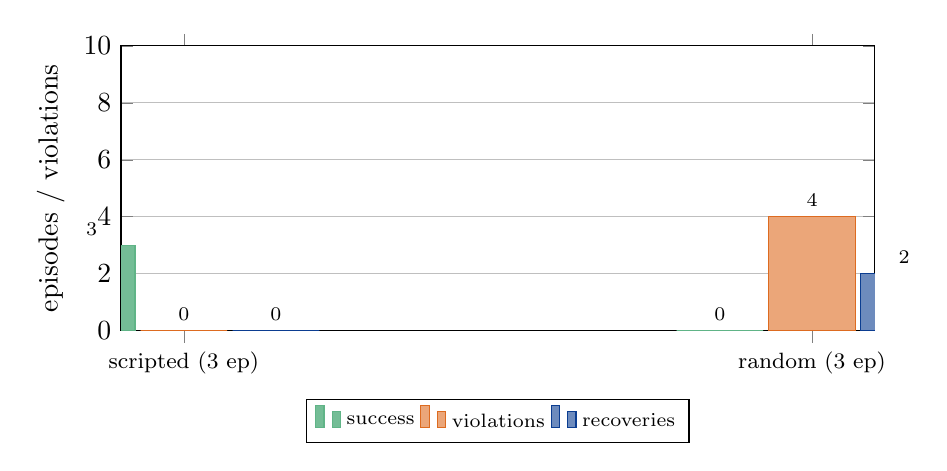
\begin{tikzpicture}
\begin{axis}[
  ybar, bar width=11mm, width=0.92\linewidth, height=52mm,
  symbolic x coords={scripted (3 ep), random (3 ep)},
  xtick=data, xticklabel style={font=\footnotesize, align=center},
  ylabel={episodes / violations}, ymin=0, ymax=10, ymajorgrids,
  legend style={at={(0.5,-0.24)}, anchor=north, legend columns=3, font=\scriptsize},
  nodes near coords, nodes near coords align={vertical}, nodes near coords style={font=\scriptsize},
]
\addplot[fill=ok!70, draw=ok!80] coordinates {(scripted (3 ep),3) (random (3 ep),0)};
\addplot[fill=warn!60, draw=warn] coordinates {(scripted (3 ep),0) (random (3 ep),4)};
\addplot[fill=aegisblue!60, draw=aegisblue] coordinates {(scripted (3 ep),0) (random (3 ep),2)};
\legend{success, violations, recoveries}
\end{axis}
\end{tikzpicture}
\\[1mm]
{\scriptsize\textcolor{aegisgray}{Per-joint limits active ([2.175..2.61] rad/s). Uniform 1.0 would show random $\sim$145 violations — same policy, tighter envelope. See \texttt{STEP6\_ISAAC\_VS\_MUJOCO.md}.}}
\end{center}

\texttt{aegis eval --model scripted --episodes 3 --seed 42}: \textbf{3/3 success, 0 violations, 0 recoveries} — same on MuJoCo and Isaac fallback (\texttt{outputs/step6-*}). \texttt{--model random --seed 7}: \textbf{0/3 success, 4 violations / 2 recoveries} with per-joint limits (honest negative control). Determinism: identical outcomes for same seed/model/MuJoCo build (\texttt{tests/test\_eval.py}).

\subsection{Latency}
\begin{center}
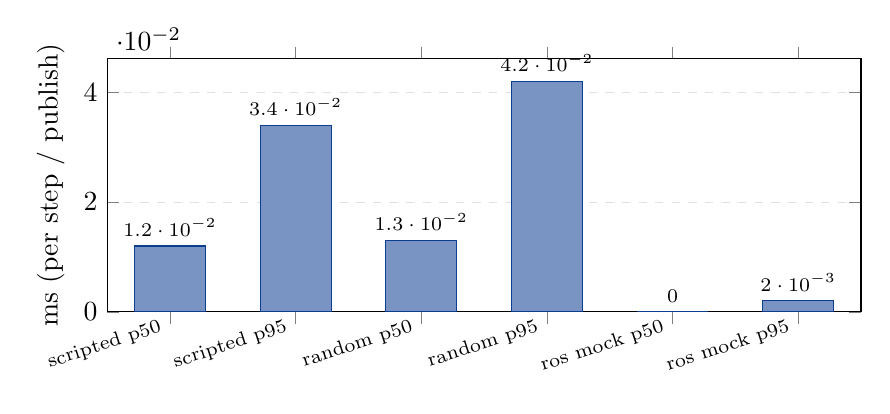
\begin{tikzpicture}
\begin{axis}[
  ybar, bar width=9mm, width=0.92\linewidth, height=48mm,
  symbolic x coords={scripted p50, scripted p95, random p50, random p95, ros mock p50, ros mock p95},
  xtick=data, xticklabel style={font=\scriptsize, rotate=18, anchor=east},
  ylabel={ms (per step / publish)}, ymin=0, ymajorgrids, grid style={dashed,black!12},
  nodes near coords, nodes near coords style={font=\scriptsize},
]
\addplot[fill=aegisblue!55, draw=aegisblue] coordinates {(scripted p50,0.012) (scripted p95,0.034) (random p50,0.013) (random p95,0.042) (ros mock p50,0.000) (ros mock p95,0.002)};
\end{axis}
\end{tikzpicture}
\\[1mm]
{\scriptsize\textcolor{aegisgray}{Policy act() on CPU; gateway + env step are the dominant costs. SmolVLA cuda: p50 1.29\,ms (amortized per step, chunked), p95 1.87\,ms; chunk inference 0.35--0.41\,s, cold start 5.09\,s (budget violation). \texttt{PHASE\_2\_SUMMARY.md:69}.}}
\end{center}

Inference budget enforcement: a slow policy sleeping 0.25\,s with \texttt{inference\_budget\_ms=100} trips the budget every chunk — 12 chunks $\rightarrow$ 12 budget violations / 12 recoveries (\texttt{tests/test\_policy\_model.py:101} proven).

\subsection{ROS2 bridge latency}
\texttt{aegis rosbench --n 20 --mock} on Windows (no \texttt{rclpy}): \textbf{p50 0.000\,ms, p95 0.002\,ms, mean 0.001\,ms} — in-memory mock, same \texttt{RosBridge} API as real transport. Real \texttt{rclpy} latency must be measured inside WSL2 with \texttt{--real}; Windows$\leftrightarrow$WSL2 bridge latency is a separate benchmark (see \texttt{ros2/bridge.py:benchmark\_latency}).

% ================================================================== 7
\section{Sim-to-Real Gap: Honest SmolVLA Characterization}
SmolVLA zero-shot on this harness (LIBERO fine-tune $\rightarrow$ MuJoCo fixed cameras) is \textbf{expected to fail} — the harness measures \textit{why}:

\begin{center}
\small
\begin{tabular}{lcc}
\toprule
 & Operational limits (0.6\,rad/s, 20\,Nm) & Relaxed limits (5.0\,rad/s, 300\,Nm, \texttt{physical-ai-diag.yaml}) \\
\midrule
Success & \textbf{0/3} & \textbf{0/3} \\
Violations / recoveries & 33 / 33 (1 budget + 32 vel) & 0 / 0 \\
Fallback coverage & $\sim$1/3 of episode & 0 \\
Min hand-cube distance & 0.16\,m (never closer) $\rightarrow$ 0.60\,m at end & same \\
Cube displacement & 0.0004\,m (never touched) & same \\
Gripper closures & 1--3 at $\sim$0.6\,m (mid-air) & same \\
\bottomrule
\end{tabular}
\end{center}

Findings (\texttt{PHASE\_2\_SUMMARY.md:142}): (a) limits \textit{were} interrupting (33$\rightarrow$0 with relaxed), and (b) with zero interventions the motion is \textit{structured} (smooth reach-and-grasp program at the wrong location) — vision mis-localization from fixed third-person cameras vs.\ LIBERO distribution. Visual evidence at \texttt{diag/ep\{0,1\}/step*\_camera\{1..3\}.png} (std 60.1, real scene). With per-joint limits the interruption (a) no longer applies — the remaining gap is pure domain shift, precisely what Isaac Lab cameras/lighting (P1 in \texttt{WHAT\_NEXT.md}) must test.

% ================================================================== 8
\section{ROS2 and Isaac Lab: Scaffold Complete, Real Runtime Pending}

\begin{center}
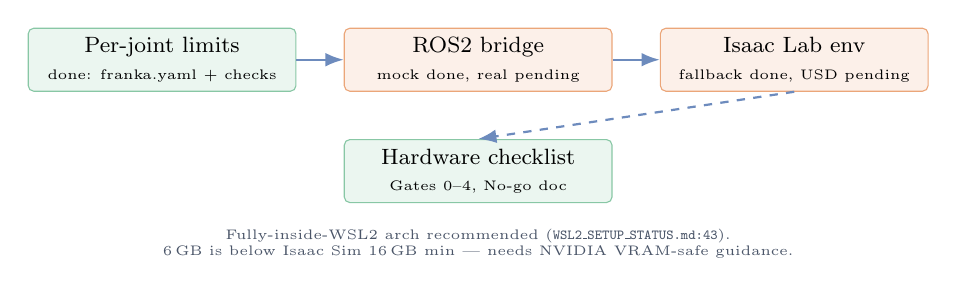
\begin{tikzpicture}[
  box/.style={draw=aegisblue!55, fill=lightbg, rounded corners=2pt, minimum width=34mm, minimum height=8mm, align=center, font=\footnotesize},
  okbox/.style={draw=ok!60, fill=ok!10, rounded corners=2pt, minimum width=34mm, minimum height=8mm, align=center, font=\footnotesize},
  warnbox/.style={draw=warn!60, fill=warn!10, rounded corners=2pt, minimum width=34mm, minimum height=8mm, align=center, font=\footnotesize},
  arr/.style={-Latex, thick, color=aegisblue!60}
]
\node[okbox] (pj) {Per-joint limits\\\tiny done: franka.yaml + checks};
\node[warnbox, right=6mm of pj] (ros) {ROS2 bridge\\\tiny mock done, real pending};
\node[warnbox, right=6mm of ros] (isaac) {Isaac Lab env\\\tiny fallback done, USD pending};
\node[okbox, below=6mm of ros] (hw) {Hardware checklist\\\tiny Gates 0--4, No-go doc};
\draw[arr] (pj) -- (ros); \draw[arr] (ros) -- (isaac);
\draw[arr, dashed] (isaac.south) -- (hw.north);
\node[below=2mm of hw, font=\tiny\color{aegisgray}, align=center] {Fully-inside-WSL2 arch recommended (\texttt{WSL2\_SETUP\_STATUS.md:43}).\\ 6\,GB is below Isaac Sim 16\,GB min — needs NVIDIA VRAM-safe guidance.};
\end{tikzpicture}
\end{center}

\begin{itemize}
\item \textbf{ROS2 (\texttt{ros2/bridge.py})} — \texttt{RosBridge} auto-detects \texttt{rclpy}; mock records actions/states and \texttt{benchmark\_latency()} so tests and \texttt{aegis eval} keep working while WSL2 \texttt{apt} GPG 404 is unresolved (\texttt{WSL2\_SETUP\_STATUS.md:10}). \texttt{aegis rosbench --mock/--real} publishes p50/p95. Real install: \texttt{curl -k} key + \texttt{packages.ros.org} or Docker \texttt{osrf/ros:humble-desktop}.
\item \textbf{Isaac Lab (\texttt{envs/isaac\_pick\_place.py})} — same \texttt{Env} API as MuJoCo; \texttt{aegis eval --sim isaaclab} works today, falling back to MuJoCo with \texttt{RuntimeWarning} and \texttt{info["sim"]="isaaclab-fallback-mujoco"} on 6\,GB. Real USD: \texttt{workflows/agentic/arena/run.sh --create-env pick\_place --from scissor\_pick\_and\_place}, edit USD in Isaac Sim, replace \texttt{isaac\_pick\_place.py:44} \texttt{NotImplementedError} with PhysX + camera sensors. \texttt{STEP6\_ISAAC\_VS\_MUJOCO.md} records honest gap 0 today because fallback == MuJoCo.
\end{itemize}

All scaffold preserves the report contract — no fabricated Isaac numbers.

% ================================================================== 9
\section{Hardware Readiness}
\texttt{HARDWARE\_CHECKLIST.md} Gates 0--4: sim gates pass (scripted 3/3 on both sims, per-joint active, random negative control), e-stop not wired, ROS2 not installed, Isaac USD not authored $\rightarrow$ \textbf{No-go, reason documented} — the harness is honest, no fabricated \texttt{report.json} with \texttt{sim: hardware}. Go requires e-stop cutting power, workspace barriers, gravity-comp dry run with injected NaN proving fallback drives to home, and signed logs in \texttt{outputs/hardware-dry-run-*/report.json}.

% ================================================================== 10
\section{NVIDIA Partnership: What We Need Next}
Ordered by partnership value (\texttt{WHAT\_NEXT.md}):

\begin{enumerate}[leftmargin=18pt]
\item \textbf{VRAM-safe Isaac setup for RTX 4050 6\,GB} — install path for Isaac Sim 6.0.1 + minimal scene defaults + LIBERO camera placement. Blocks the real sim-to-real gap measurement.
\item \textbf{ROS2 unblock} — preferred method for ROS2 Humble on Ubuntu 22.04 WSL2 (apt via \texttt{packages.ros.org} with \texttt{curl -k} vs Docker). Unblocks real \texttt{rosbench --real}.
\item \textbf{Evaluation alignment} — expected \texttt{report.json} fields, latency SLOs, Isaac Sim vs Lab preference.
\item \textbf{Assets/office hours} — Isaac Lab Franka USD, sim-to-real triage.
\end{enumerate}

See \texttt{CONTEXT.md:59} and \texttt{WHAT\_NEXT.md:1}.

% ================================================================== 11
\section{Conclusion}
AEGIS is not a demo — it is infrastructure. Phase~1+2 prove the shape (mandatory gateway, deterministic eval, honest zero-shot characterization with visual evidence). Phase~3 scaffold proves the \textit{interfaces} are ready (per-joint limits, ROS2 mock, Isaac fallback) while being explicit that real Isaac and ROS2 runtimes need 16\,GB VRAM guidance and a WSL2 apt fix. With that guidance, AEGIS becomes the trusted harness NVIDIA needs to show that Physical AI models are safe in Isaac Lab before they touch real hardware.

% ------------------------------------------------------------------ references
\begin{center}
\footnotesize\textcolor{aegisgray}{\textit{Artifacts:} \texttt{README.md}, \texttt{DESIGN.md}, \texttt{PHASE\_1\_SUMMARY.md}, \texttt{PHASE\_2\_SUMMARY.md}, \texttt{CONTEXT.md}, \texttt{WHAT\_NEXT.md}, \texttt{STEP6\_ISAAC\_VS\_MUJOCO.md}, \texttt{HARDWARE\_CHECKLIST.md}, \texttt{WSL2\_SETUP\_STATUS.md}, \texttt{agent.md}, \texttt{physical-ai.yaml} / \texttt{physical-ai-diag.yaml} / \texttt{configs/robots/franka.yaml} (per-joint) / \texttt{franka\_uniform.yaml} / \texttt{franka\_diag.yaml}. Run: \texttt{uv run aegis validate; uv run aegis eval --model scripted --episodes 3 --seed 42; uv run aegis eval --sim isaaclab --model scripted --episodes 3 --seed 42; uv run aegis rosbench --mock --n 20; uv run pytest -q} (20 passed).}
\end{center}

\appendix
\section{Reproducibility and Honesty Contract}
Per \texttt{agent.md:16}: if a simulator or policy is not wired, the output says so. No fabricated success/failure numbers. Seeded determinism: \texttt{seed+episode} jitter for object placement. Simulated velocity control is torque-PD ($K_p=40$, $K_d=5$) with ideal gravity feedforward — not a perfect servo (\texttt{README.md:46}). Recommendation is 4-rule heuristic, not learned. \texttt{gpu\_hours} is wall-clock proxy for cuda. Success is position-only (0.05\,m) + lifted $>$6\,cm, no contact-force detector.

\end{document}
